\section{Theorie}
\label{sec:Theorie}

\subsection{Allgemeine Brückenschaltung}

\begin{figure}
    \centering
    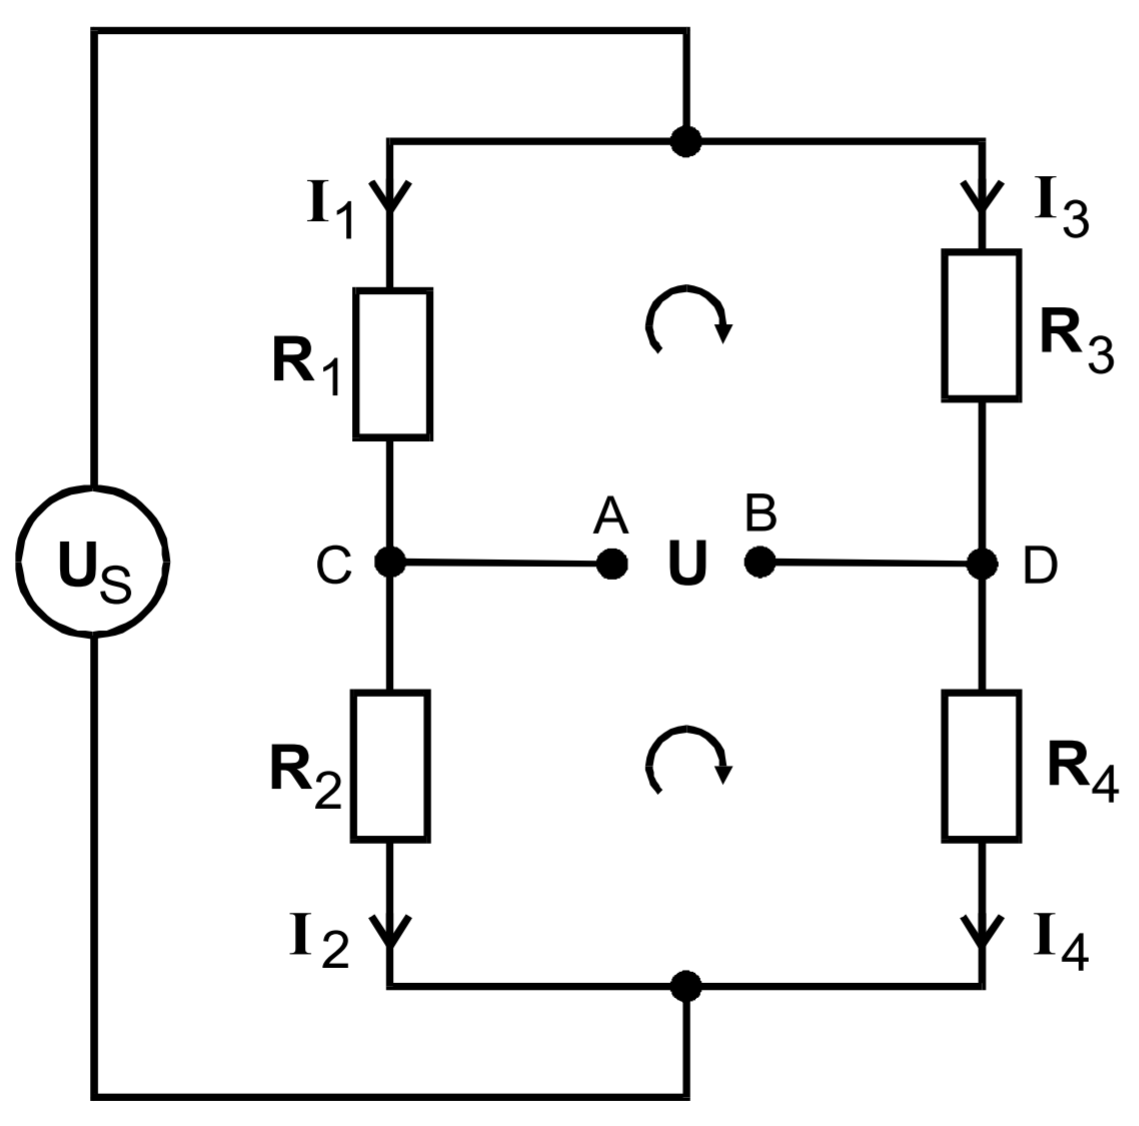
\includegraphics[width=0.5\textwidth]{pictures/Schaltung1.png}
    \caption{Ein beispielhafter Aufbau einer einfachen Brückenschaltung \cite[1]{v302}.}
    \label{fig:Schaltung1}
\end{figure}

Brückenschaltungen sind essentiell, wenn unbekannte Widerstände bestimmt werden sollen.
Um mit einer Brückenschaltung, beispielsweise wie in Abbildung \ref{fig:Schaltung1},
benötigt man eine bakannte Speisespannung $U_\text{S}$ und vier Widerstände.
Durch alle Widerstände wird ein Strom fließen.
Es gelten die \textit{Kirchhoffschen Regeln}.
Es gilt für die Summe aller Ströme an einem Knotenpunkt
\begin{equation} \label{eq:kirch1}
    \sum_k I_k = 0 \, ,
\end{equation}
und für die Summe der Spannungen in einem abgeschlossenen Stromkreis
\begin{equation} \label{eq:kirch2}
    \sum_k U_k = 0 \, .
\end{equation}

Durch diese Regeln lässt sich die Formel für die Brückenspannung, die an den Punkten $A$ und $B$ abgegriffen wird,
angeben. Diese lautet
\begin{equation}
    U_\text{Brück} = \frac {R_2 R_3 - R_1 R_4} {(R_3 + R_4)(R_1 + R_2)} U_\text{S} \, .
\end{equation}

Es kann durchaus der Fall auftreten, oder willentlich bewirkt werden, dass die Brückenspannung vollständig verschwindet.
In diesem Falle gilt
\begin{equation} \label{eq:Brückenspannunggleich0}
    R_2 R_3 = R_1 R_4 \, .
\end{equation}

\subsection{Wheatstonesche Brücke}

\begin{figure}
    \centering
    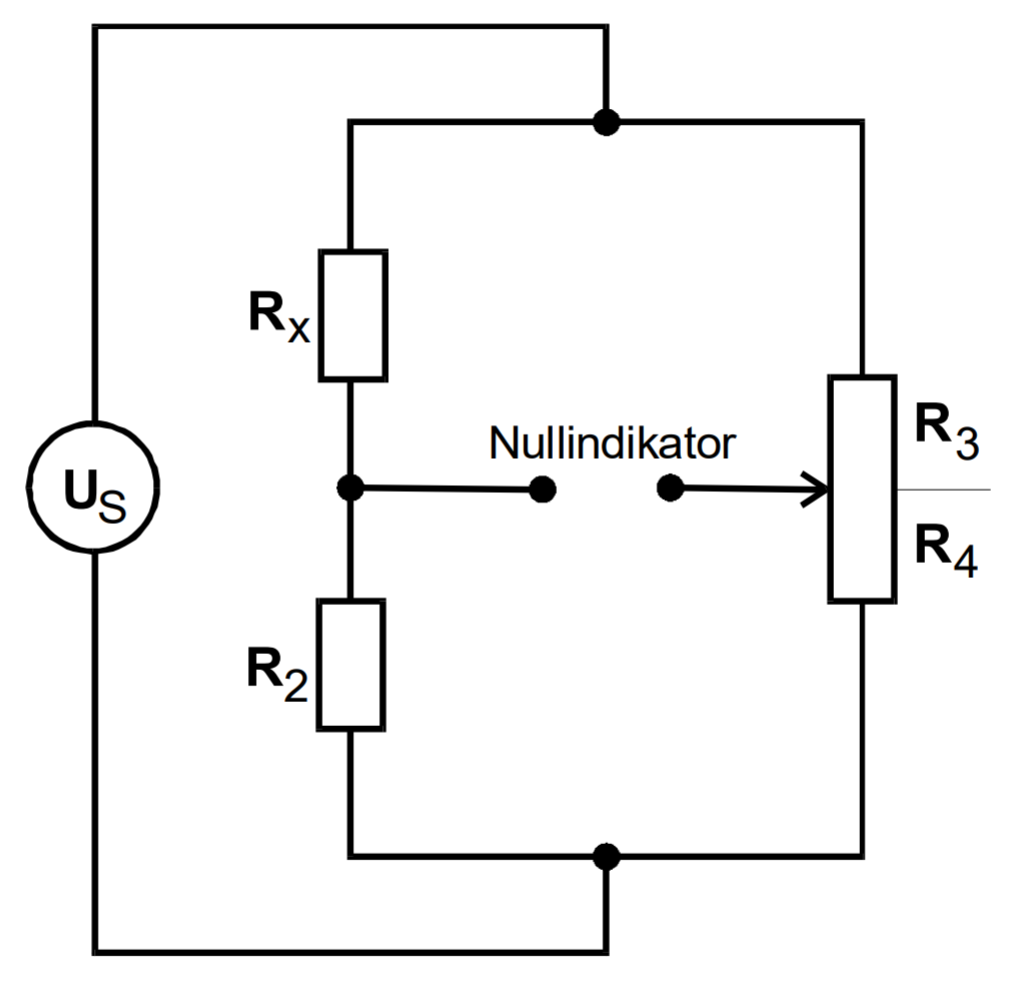
\includegraphics[width=0.5\textwidth]{pictures/Schaltung2.png}
    \caption{Die Wheatstonesche Brückenschaltung \cite[4]{v302}.}
    \label{fig:Schaltung2}
\end{figure}

Mit der Wheatstonschen Brückenschaltung lassen sich besonders einfach unbekannte ohmsche Widerstände bestimmen.
Die Schaltung ist analog zu der in Abbildung \ref{fig:Schaltung1}, mit der Ausnahme das $R_1$ nun durch einen unbekannten Widerstand
$R_x$ ersetzt wird.
Durch die Gleichung (\ref{eq:Brückenspannunggleich0}) erhält man dann 
\begin{equation} \label{eq:Rx}
    R_x = \frac {R_2 R_3}{R_4} \, .
\end{equation}
Anstelle von $R_3$ und $R_4$ kann ebenfalls ein Potentiometer benutzt werden.

\subsection{Kapazitätsmessbrücke}

\begin{figure}
    \centering
    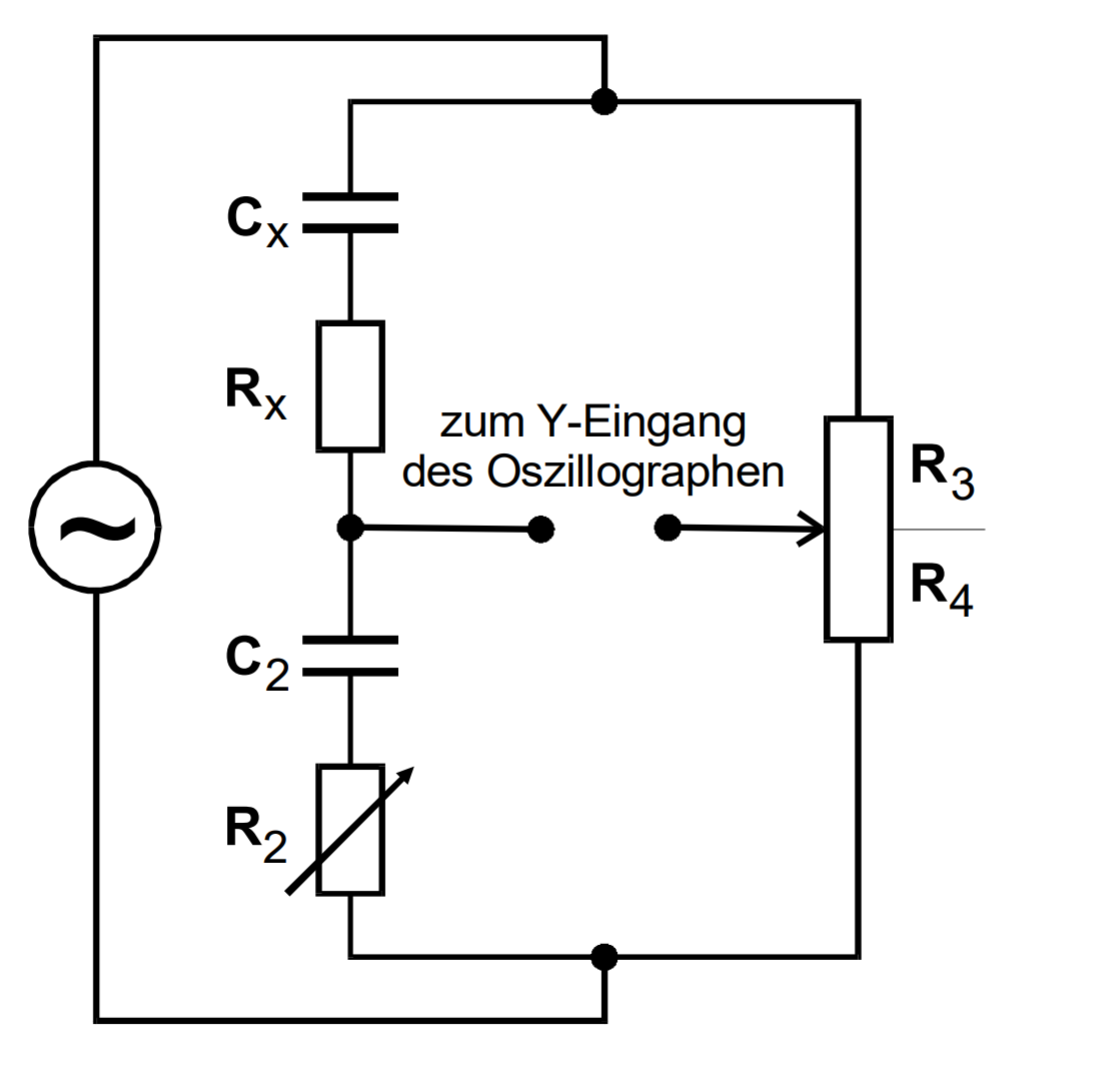
\includegraphics[width=0.5\textwidth]{pictures/Schaltung3.png}
    \caption{Eine Kapazitätmessbrücke mit unbekanntem ohmschen und kapazitiven Widerstand \cite[5]{v302}.}
    \label{fig:Schaltung3}
\end{figure}

\subsection{Induktivitätsmessbrücke}

\begin{figure}
    \centering
    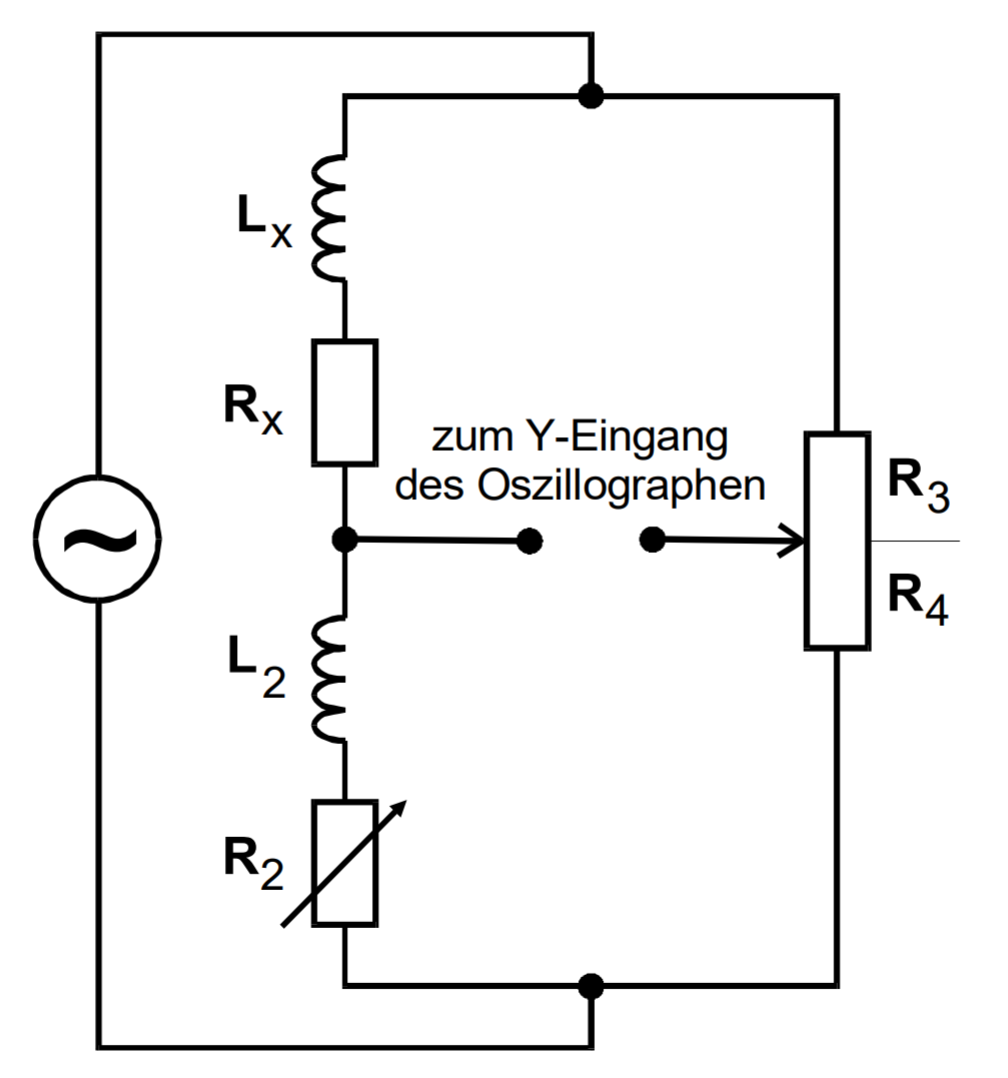
\includegraphics[width=0.5\textwidth]{pictures/Schaltung4.png}
    \caption{Die Induktivitätsmessbrücke mit unbekanntem ohmschen und induktiven Widerstand \cite[6]{v302}.}
    \label{fig:Schaltung4}
\end{figure}

\subsection{Maxwell Brücke}
\begin{figure}
    \centering
    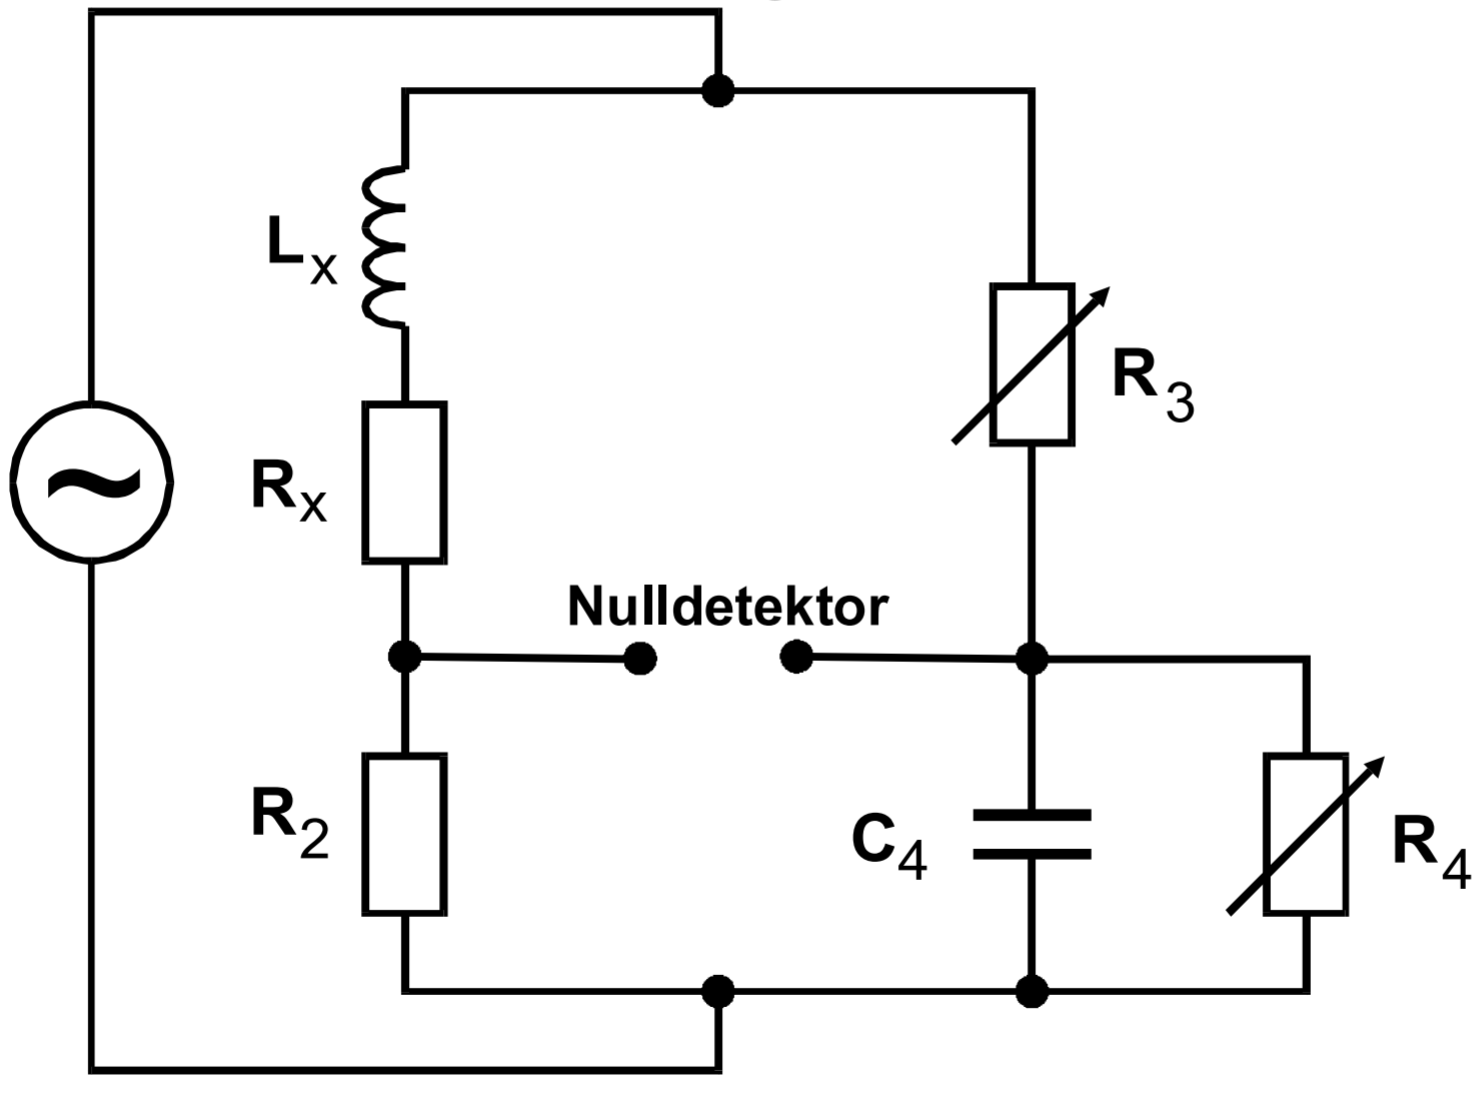
\includegraphics[width=0.5\textwidth]{pictures/Schaltung5.png}
    \caption{Eine Maxwellsche Brückenschaltung zur Messung eines ohmschen und induktiven Widerstandes \cite[7]{v302}.}
    \label{fig:Schaltung5}
\end{figure}


\subsection{Wien-Robinson-Brücke}

\begin{figure}
    \centering
    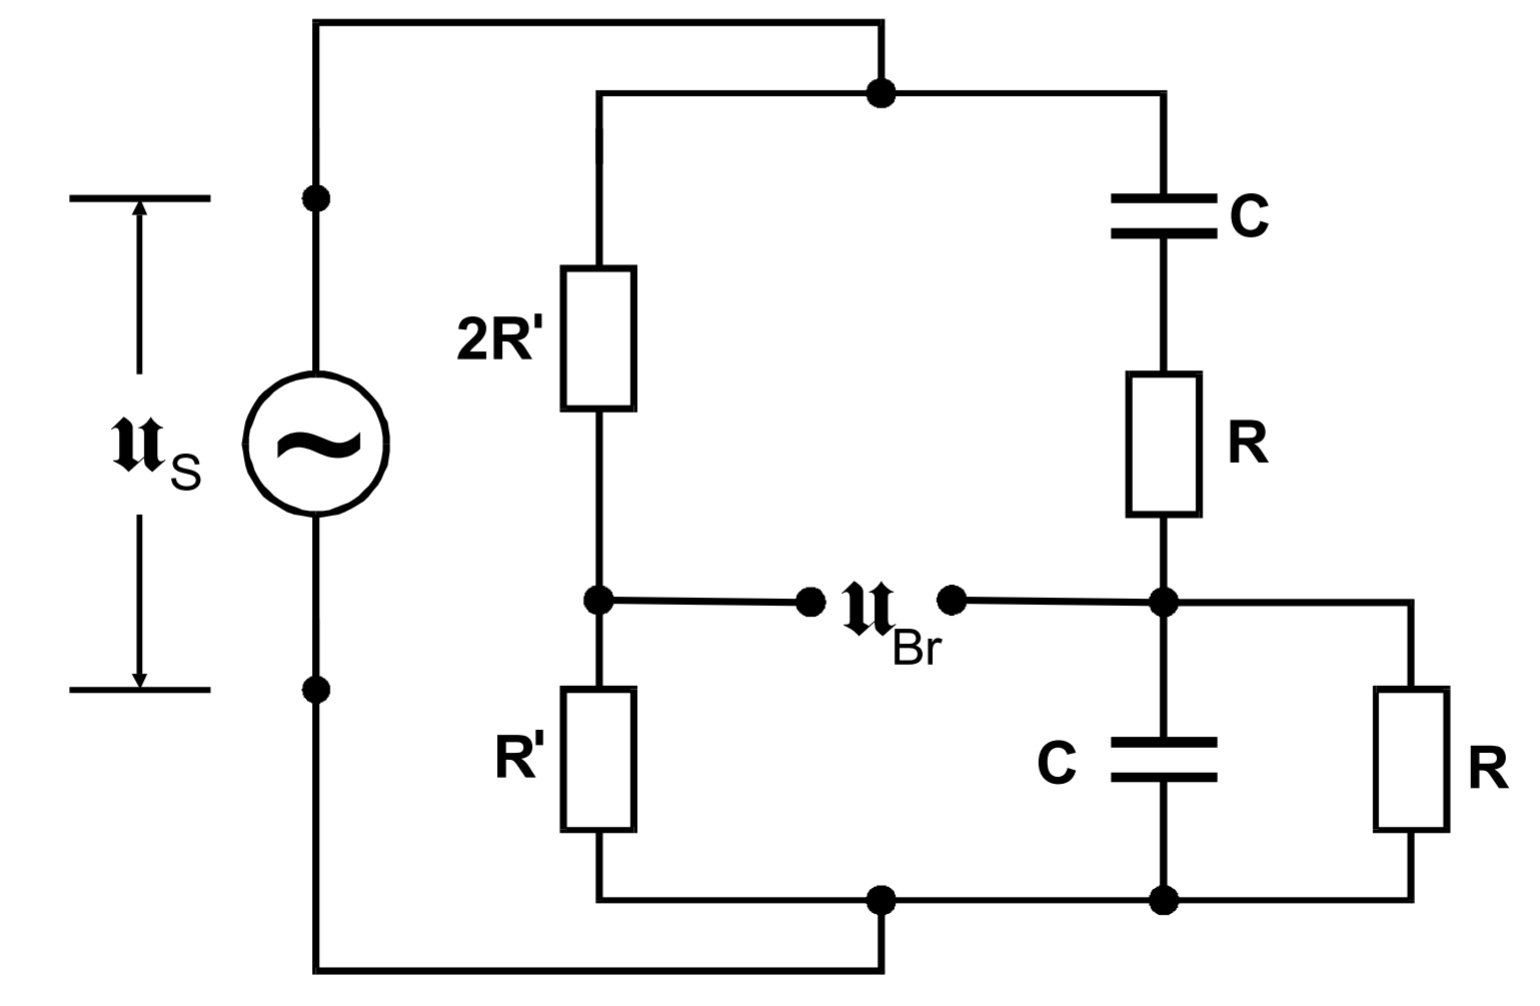
\includegraphics[width=0.5\textwidth]{pictures/Schaltung6.png}
    \caption{Die Wien-Robinson-Brücke \cite[8]{v302}.}
    \label{fig:Schaltung6}
\end{figure}

